\subsection{Slučaj upotrebe: Pregled informacija o izborima}

\subsubsection*{Kratak opis}
Student pregleda raspisane izbore, period glasanja i izborne liste koje učestvuju na izborima, kao i informaciju o tome da li ima pravo glasa.

\subsubsection*{Akteri}
\begin{itemize}
    \item \textbf{Student} -- pregleda informacije o izborima i izbornim listama.
\end{itemize}

\subsubsection*{Preduslovi}
\begin{itemize}
    \item Student je prijavljen u sistem.
\end{itemize}

\subsubsection*{Postuslovi}
\begin{itemize}
    \item Student je upoznat sa periodom glasanja, izbornim listama i svojim pravom glasa.
    \item Stanje sistema se ne menja.
\end{itemize}

\subsubsection*{Osnovni tok}
\begin{enumerate}
    \item Student bira opciju \textbf{Izbori}.
    \item Sistem prikazuje spisak izbora sa periodom glasanja i statusom (\textit{najavljeni}, \textit{u toku}, \textit{završeni}).
    \item Student bira izbore.
    \item Sistem prikazuje detalje izbora i spisak izbornih lista sa nosiocima i opisom programa.
    \item Sistem prikazuje da li student ima pravo glasa na izabranim izborima i da li je već glasao.
    \item Student pregleda informacije o izbornim listama.
\end{enumerate}

\subsubsection*{Alternativni tokovi}
\begin{enumerate}[label=\textbf{A\arabic*.}]
    \item \textbf{Nema raspisanih izbora.} Ako u koraku 2 u sistemu ne postoje objavljeni izbori, sistem prikazuje poruku da trenutno nema raspisanih izbora. Slučaj upotrebe se završava.
    \item \textbf{Prelazak na glasanje.} Ako je glasanje u toku, a student ima pravo glasa i još nije glasao, student u koraku 6 može da izabere opciju \textbf{Glasaj}. Tada počinje slučaj upotrebe \textit{Elektronsko glasanje}.
\end{enumerate}

\begin{figure}[H]
    \centering
    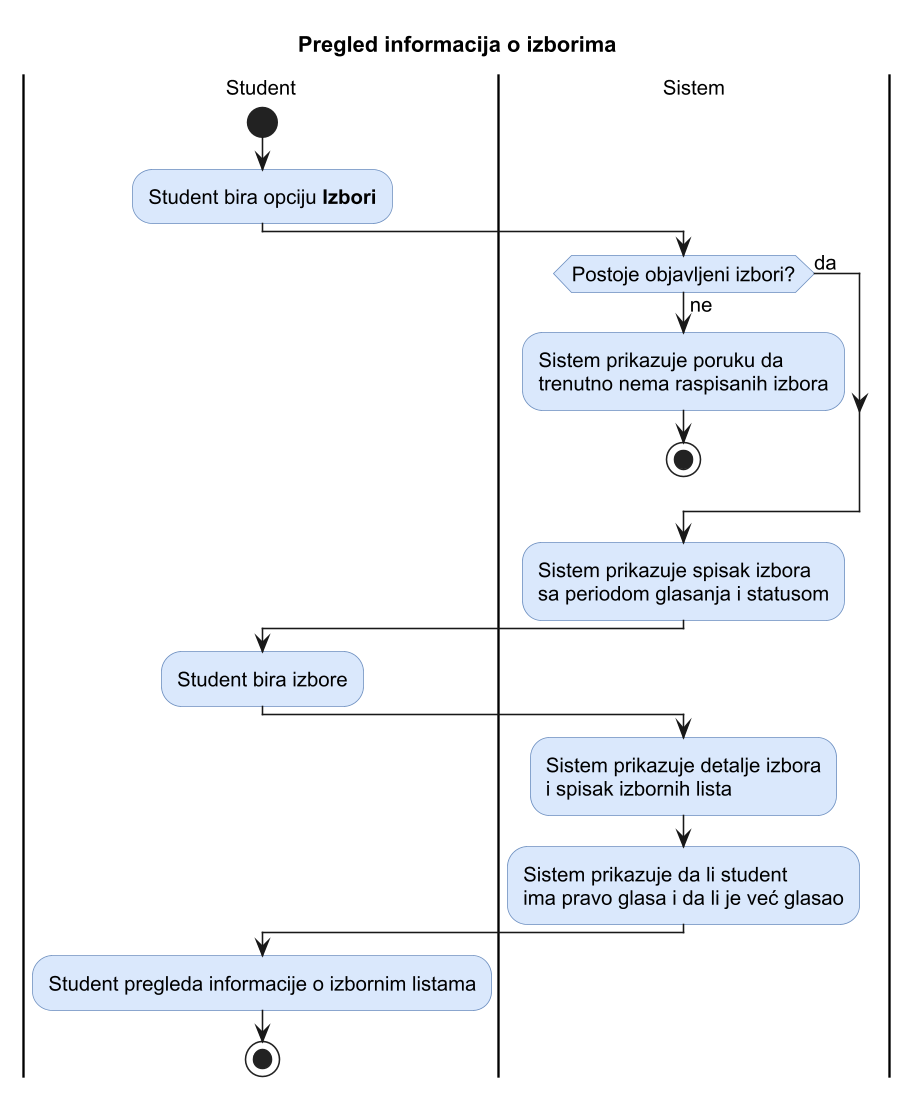
\includegraphics[width=0.7\textwidth]{aktivnosti_pregled_informacija.png}
    \caption{Dijagram aktivnosti: Pregled informacija o izborima}
    \label{fig:pregled_informacija}
\end{figure}

\newpage
